\documentclass[../../thesis.tex]{subfiles}

\begin{document}
\begin{figure}[ht]
    \centering
    \pgfdeclarelayer{bg}    % declare background layer
    \pgfsetlayers{bg,main}  % set the order of the layers (main is the standard layer)
    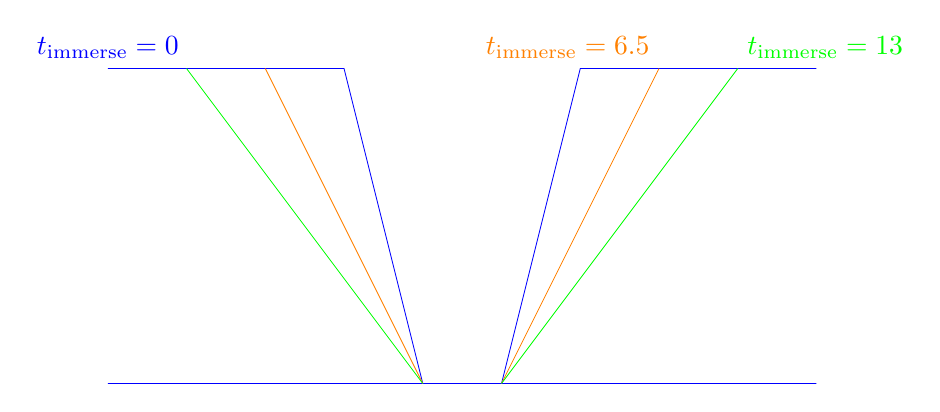
\begin{tikzpicture}
        \draw[line width=0.3,color=blue] (0,0)--(4,0)--(3,4)--(0,4) node[anchor=south] {$t_\mathrm{immerse}=\SI{0}{\minute}$};
        \draw[line width=0.3,color=blue] (9,0)--(5,0)--(6,4)--(9,4);
        \draw[line width=0.3,color=blue] (4,0)--(5,0);
        \draw[line width=0.3,color=orange] (4,0)--(2,4);
        \draw[line width=0.3,color=orange] (5,0)--(7,4) node[anchor=south east] {$t_\mathrm{immerse}=\SI{6.5}{\minute}$};
        \draw[line width=0.3,color=green] (4,0)--(1,4);
        \draw[line width=0.3,color=green] (5,0)--(8,4) node[anchor=south west] {$t_\mathrm{immerse}=\SI{13}{\minute}$};
    \end{tikzpicture}
    \caption{Immersion of a closed pore membrane resulting in an increase of the funnelling aspect of the pores due to the saturation of the acid within the pores. The visualized theory is backed by the isotherms in \cref{fig:immersed-comp-w296} and explained in \cref{subsec:immersed-membranes}.}
    \label{fig:wafer_295}
\end{figure}
\end{document}
